\subsubsection{Properties}

\begin{enumerate}
    \item \textbf{Every tree with $n$ nodes has $n-1$ edges}.
    \begin{proof}[Inductive proof]
        Base case: the claim holds for $n=1$ (tree with $1$ node and $0$ edges).

        Inductive step: show that, if this is true for trees with $n$ nodes, then it is also true for those with $n+1$ nodes.

        Let $T_{1}$ be a tree with $n+1$ nodes and recall that any tree with $n \ge 2$ nodes has at least $2$ leaves (two nodes of degree 1, the number of incident edges). By deleting one leaf and its incident edge, we obtain a tree $T_{2}$ with $n$ nodes. By induction hypothesis, $T_{2}$ has $n-1$ edges. Therefore, the tree $T_{1}$ has $n-1+1 = n$ edges.
    \end{proof}

    \item \textbf{Every pair of nodes in a tree is connected by a unique path}. The proof is not necessary, because otherwise there would be a cycle (and this is against the definition of a tree).

    \item \textbf{By adding a new edge to a tree, we can create a unique cycle}.

    \item Let $G_{T} = \left(N,T\right)$ be a spanning tree of $G = \left(N,E\right)$. Consider an edge $e \notin T$ and the unique cycle $C$ of $T \cup \left\{e\right\}$ (as in property 3). For each edge $f \in C \setminus \left\{e\right\}$, the subgraph $T \cup \left\{e\right\} \setminus \left\{f\right\}$ is also a spanning tree of $G$.
    \begin{figure}[!htp]
        \centering
        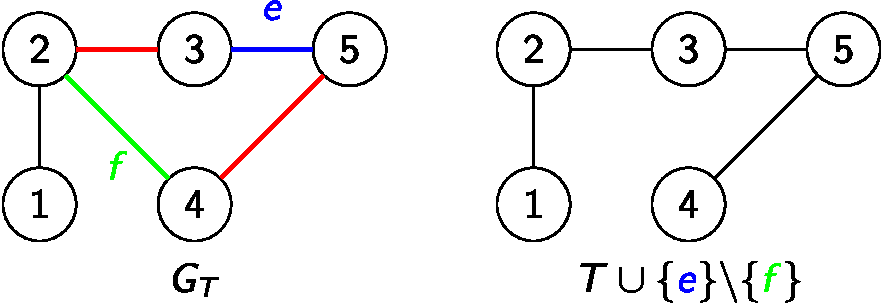
\includegraphics[width=.5\textwidth]{img/trees-5.pdf}
    \end{figure}

    \item Let $F$ be a partial tree (spanning nodes in $S \subseteq N$) contained in an optimal tree of $G$. Consider $e = \left\{u,v\right\} in \delta\left(S\right)$ of minimum cost, then there exists a minimum cost spanning tree of $G$ containing $e$ (is better explained in the \ref{paragraph: Prim's algorithm} paragraph, page \pageref{paragraph: Prim's algorithm}).

    \begin{proof}
        By contradiction, assume $T^{*} \subseteq E$ is a minimum cost spanning tree with $F \subseteq T^{*}$ and $e \notin T^{*}$. Adding edge $e$ to $T^{*}$ creates the cycle $C$. Let $f \in \delta\left(S\right) \cap C$.
        \begin{itemize}
            \item If $c_{e} = c_{f}$, then $T^{*} \cup \left\{e\right\} \setminus \left\{f\right\}$ is (also) optimal since it has same cost of $T^{*}$.
            
            \item If $c_{e} < c_{f}$, then $c\left(T^{*} \cup \left\{e\right\} \setminus \left\{f\right\}\right) < c\left(T^{*}\right)$, hence $T^{*}$ is not optimal.
        \end{itemize}
        \begin{figure}[!htp]
            \centering
            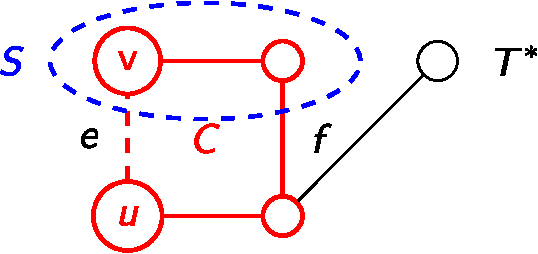
\includegraphics[width=.4\textwidth]{img/trees-9.pdf}
        \end{figure}
    \end{proof}
\end{enumerate}